\section{Simuleringsblokker}
\thispagestyle{fancy}

For å skape eit realistisk miljø for testing, lagde vi nokre simuleringsblokker.
Desse blokkene etterliknar driftssituasjonar og gjer simulering enklare og meir effektivt.
Vi lagde hovudsakleg to slike blokker, ei simulerer fylling av tank
og ei for tilbakemelding frå ventilar.

Blokk for tanksimulering er enkel og programmert spesifikt for reinseanlegget, 
som har ein mottakstank og to reaktorar.
Det er lite truleg at desse simuleringsblokkene vil bli nytta vidare, men dei gav
oss den realismen vi trengte.

Desse blokkene forenkla også sjølve arbeidet med simuleringa.
Før vi utvikla blokka for tilbakemelding på ventilar, 
gav vi manuelt kvar ventil XGH eller XGL basert på den tiltenkte stillinga (open/stengd). \newline
Dette fungerer greitt dersom ein testar ei ventilblokk, men
når simuleringa omfattar større delar av programmet blir denne jobben tidkrevjande.

På desse blokkene har vi tatt oss meir friheit i namngiving og feilhandtering, sidan blokkene ikkje skal nyttast når programmet er ferdigstilt.


\begin{figure}[htbp]
    \centering
    \begin{subfigure}[b]{0.3\textwidth}
        \centering
        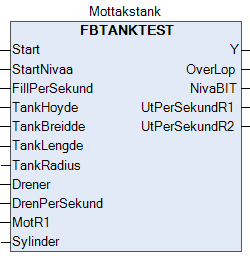
\includegraphics[width=0.9\textwidth]{Figurar/TankSim.png}
        \caption{Tank}\label{fig:TankSim}
    \end{subfigure}
    \hfill
    \begin{subfigure}[b]{0.3\textwidth}
        \centering
        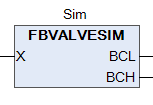
\includegraphics[width=0.9\textwidth]{Figurar/ValveSim.png}
        \caption{Ventil}\label{fig:ValveSim}
    \end{subfigure}
    \caption{Simuleringsblokker}\label{fig:SimuleringsBlokker}
\end{figure}

\newpage